\documentclass[a4paper,12pt]{article}
%%--------------------------------------------------------------------
%packages
\usepackage{zhfontcfg}
\usepackage{indentfirst}
%段前空格
\usepackage{geometry}
%利用 geometry 可以很方便的设置页面的大小
\usepackage{amsmath,amsfonts,amssymb}
%---------------------------------------------------------------------
\linespread{1.5} %行间距
\defaultfontfeatures{Mapping=tex-text}  %%如果没有它,会有一些 tex 特殊字符无法正常使用,比如连字符。
\numberwithin{equation}{section}%%公式与章节关联
\title{Win7安装过程中创建扩展分区和逻辑分区的方法}
\graphicspath{{figures/}}  

%---------------------------------------------------------------------------
\begin{document}
\maketitle
\begin{enumerate}
\item 在下面这步,按Shift+F10
 \begin{figure}[!ht]
  \centering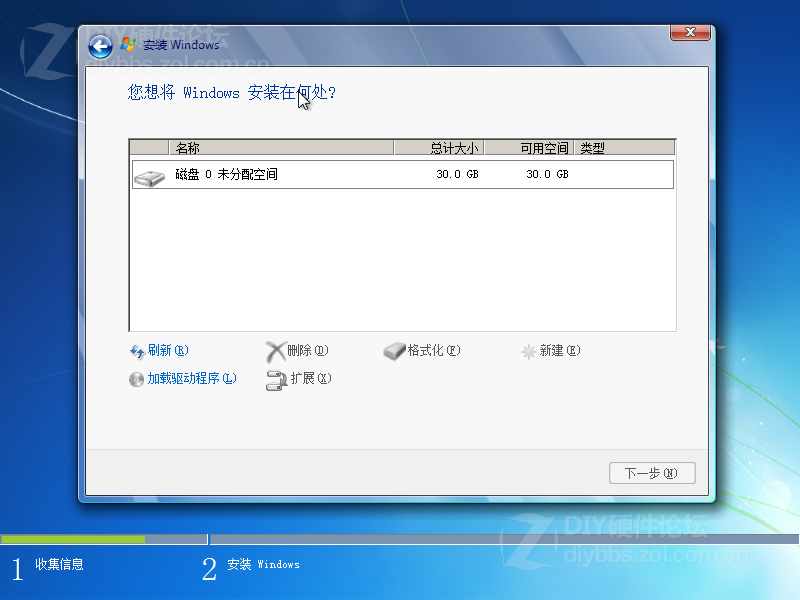
\includegraphics[width=5in]{1.png}
  \caption{1}
  \end{figure}
 \newpage

\item 输入diskpart后回车确定

 \begin{figure}[!ht]
  \centering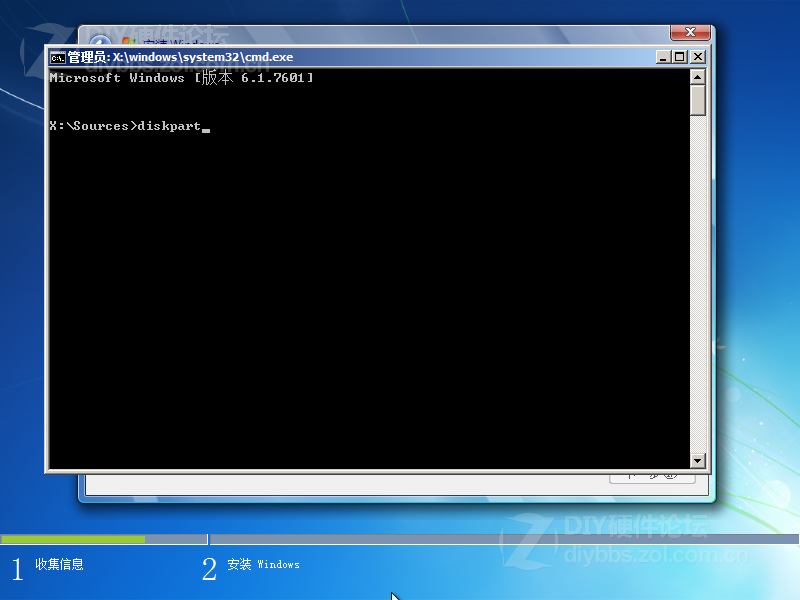
\includegraphics[width=5in]{2.png}
  \caption{2}
  \end{figure}\newpage

\item 输入list disk列出硬盘
  
 \begin{figure}[!ht]
  \centering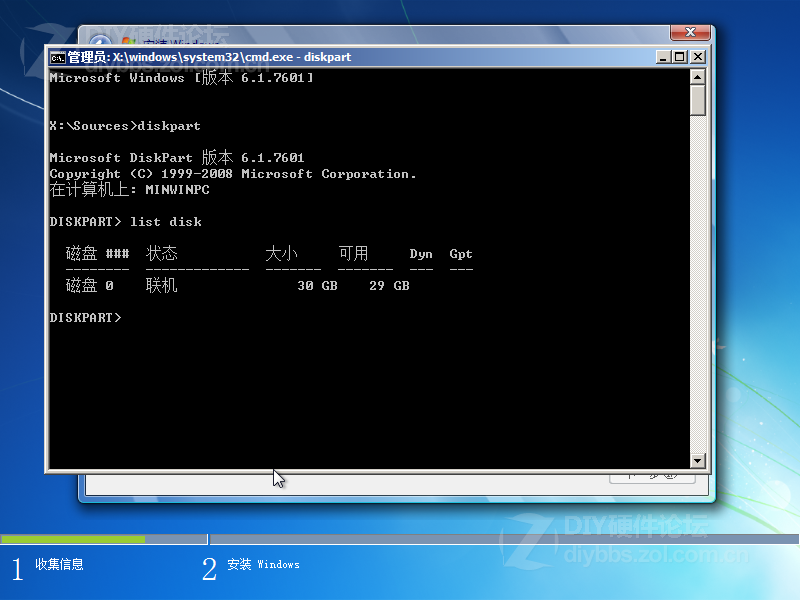
\includegraphics[width=5in]{3.png}
 \caption{3}
  \end{figure}\newpage

\item 如果你有多个硬盘,会列出0-N,这里只有一个,所以只有0,选择这个磁盘,输入:select disk 0

 \begin{figure}[!ht]
  \centering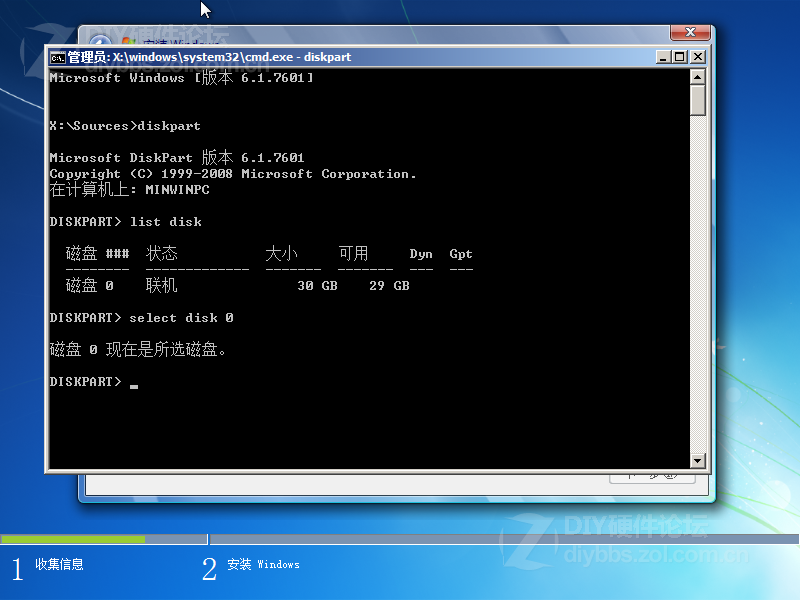
\includegraphics[width=5in]{4.png}
 \caption{4}
  \end{figure} \newpage

\item 如果你已经创建过了主分区,直接跳到下一步,如果没有创建主分区,那么输入create partition primary size=XXXX

这里XXX输入你想要创建的主分区的大小,如果这是第一个主分区,一般就是C盘了,这里是MB大小,如果输入1024MB=1G

在这里分主分区的好处就是,不会出现系统保留分区

 \begin{figure}[!ht]
  \centering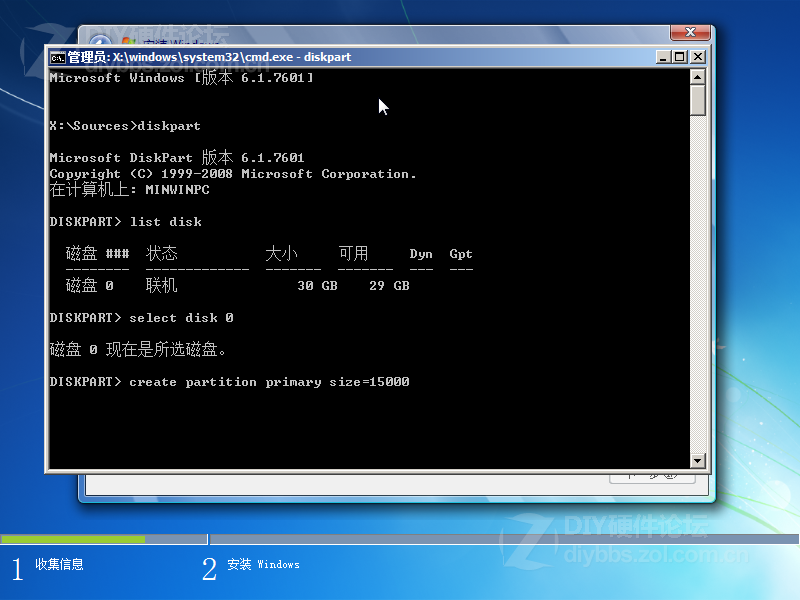
\includegraphics[width=5in]{5.png}
   \caption{5}
  \end{figure} \newpage

\item 下面是创建扩展分区输入命令:create partition extended,输入这个命令,所以剩余的未被分区的硬盘,都将变成扩展分区,如果只想分出一部分,可以参考步骤5,在create partition extended后面加上size=XXXX,如create partition extended size=100000

 \begin{figure}[!ht]
  \centering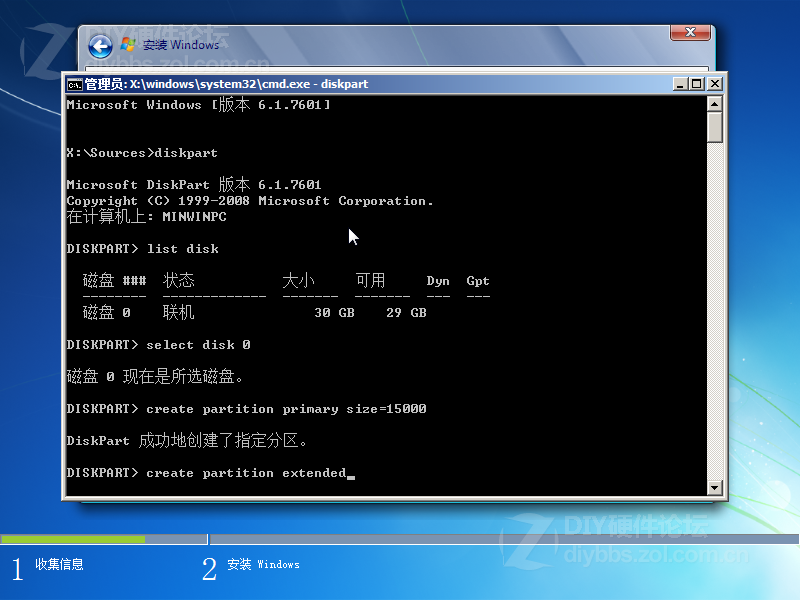
\includegraphics[width=5in]{6.png}
  \caption{6}
  \end{figure}\newpage

\item 然后关闭刚才的cmd,出现下面的图,刚才分的区没出现?不用担心,点一下刷新
 \begin{figure}[!ht]
  \centering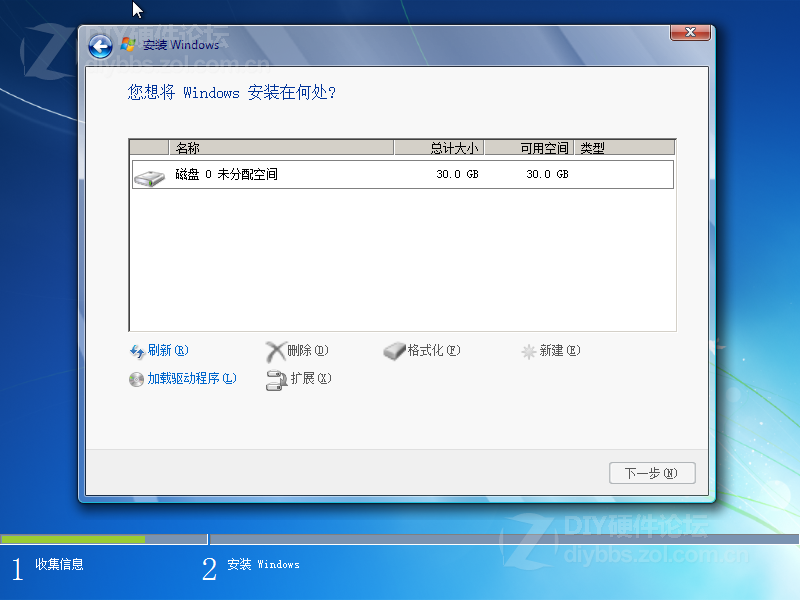
\includegraphics[width=5in]{7.png}
 \caption{7}
  \end{figure}\newpage

\item 现在已经出现刚才分的主分区和扩展分区了,但是扩展分区是不能直接用的,必须再扩展分区下面分出逻辑分区才可以,选中扩展分区,然后点新建

 \begin{figure}[!ht]
  \centering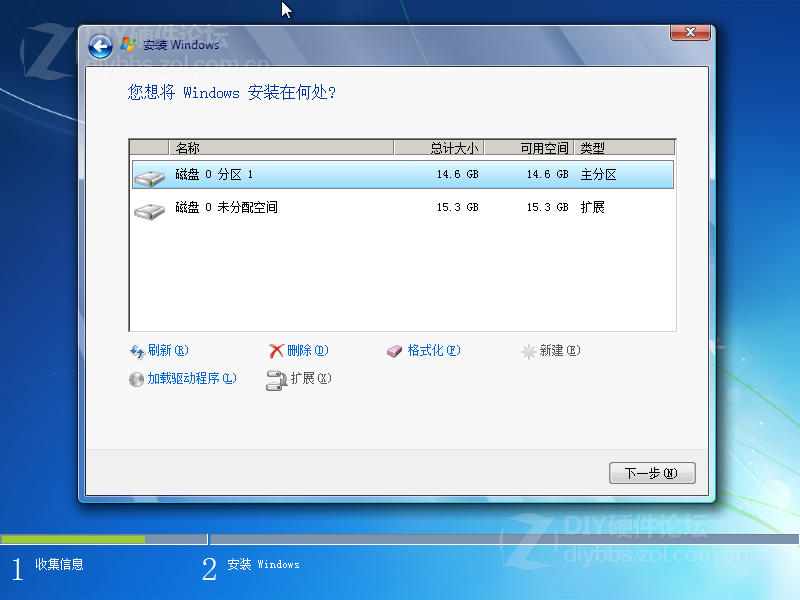
\includegraphics[width=5in]{8.png}
   \caption{8}
  \end{figure}\newpage

\item 输入你想建立一个多大的分区,大小不能超过扩展分区的总容量

\begin{figure}[!ht]
  \centering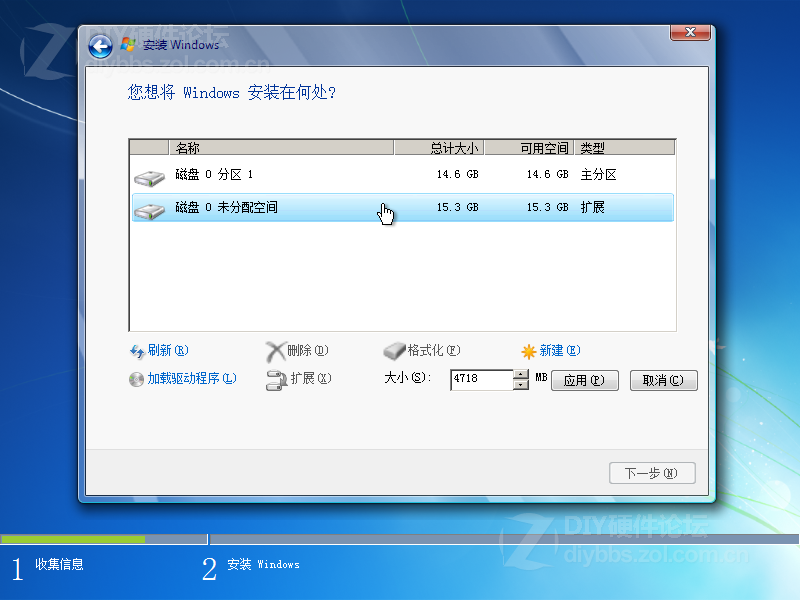
\includegraphics[width=5in]{9.png}
   \caption{9}
  \end{figure}\newpage

\item 如下图,那个15.3GB的扩展分区,被我分出了4个逻辑分区

\begin{figure}[!ht]
  \centering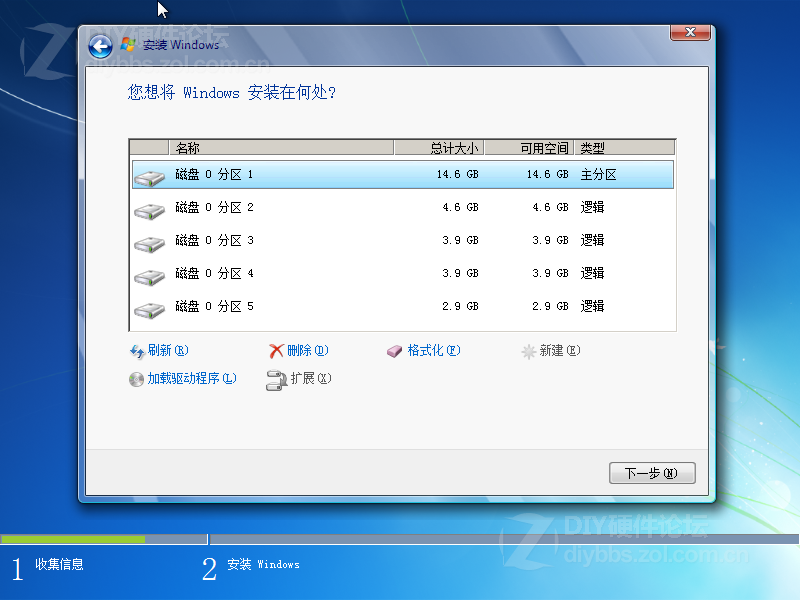
\includegraphics[width=5in]{10.png}
   \caption{10}
  \end{figure}\newpage

\end{enumerate}



\end{document}
